\documentclass[../../main.tex]{subfiles}
\begin{document}


{\bf [解]}
まずは$y=\log x$に原点$O(0,0)$から引いた接線を求めよう．
$y'=\dfrac{1}{x}$だから，点$(t,\log t)$での接線は
\begin{align}
 y = \dfrac{1}{t}\left(x-t\right) + \log t
\end{align}
である．これが原点を通るので$(x,y)=(0,0)$を代入して
\begin{align}
 0 = \log t - 1 \quad \therefore \quad t = e
\end{align}
となり，題意の接線は
\begin{align}
 y=\dfrac{1}{e}x
\end{align}
となる．よって題意の領域は下図斜線部になる．

\begin{figure}[htb]
\begin{center}
\begin{tikzpicture}[scale=1.5, >=stealth]
  % 1. 正しい領域の塗りつぶし (x軸の上側 y >= 0 のみ)
  % 0 <= x <= 1 : 接線 y = x/e と u軸 (y=0) の間
  % 1 <= x <= e : 接線 y = x/e と 曲線 y = ln(x) の間
  \begin{scope}
    \fill[pattern=north east lines, pattern color=gray!80]
      (0,0) -- (1,0) -- plot[domain=1:2.71828, samples=100] (\x, {ln(\x)}) 
      -- (2.71828, 1) -- cycle;
  \end{scope}

  % 2. 座標軸
  \draw[->] (-0.3,0) -- (3.2,0) node[right] {$x$};
  \draw[->] (0,-1.2) -- (0,1.5) node[above] {$y$};
  \node[below left] at (0,0) {$O$};

  % 3. グラフ・直線の描画
  % y = log x
  \draw[thick, domain=0.1:3.0, samples=100] plot (\x, {ln(\x)}) node[right] {$y=\log x$};
  % 接線 y = (1/e)x
  \draw[thick, domain=0:3.0] plot (\x, {\x/2.71828}) node[above left] {$y=\frac{1}{e}x$};

  % 4. 補助線 (x = e, y = 1)
  \draw[dashed] (2.71828, 0) -- (2.71828, 1) -- (0, 1);

  % 5. 交点・接点のプロット
  \fill (2.71828, 1) circle (1.2pt) node[below left] {$B$};
  \fill (2.71828, 0) circle (1.2pt) node[above left] {$A$};
  \fill (1, 0) circle (1.2pt);

  % 6. ラベル
  \node[below right] at (1,0) {$1$};
  \node[below] at (2.71828,0) {$e$};
  \node[left] at (0,1) {$1$};

\end{tikzpicture}
\end{center}
\caption{$y=\log x$ および接線 $y=\dfrac{1}{e}x$ ，$x$軸で囲まれた領域（斜線部）}
\end{figure}

題意の体積 $V$ は$O(0,0), A(e,0), B(e,1)$を頂点とする三角形の回転体から$y=\log x, y=0, x=e$に囲まれた領域の回転体の体積を減じたもので
\begin{align}
V &= 
  \left( \text{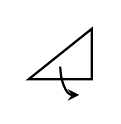
\begin{tikzpicture}[baseline={(0,-0.2)}, scale=0.8, >=stealth]
    % 直角三角形
    \draw[thick] (0,0) -- (1,0) -- (1,0.8) -- cycle;
    % 回転を表す矢印（手書きのイメージ）
    \draw[->, thick] (0.5, 0.2) to[out=-90, in=180] (0.8, -0.25);
  \end{tikzpicture}} \right)
  - 
  \left( \text{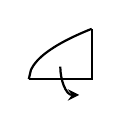
\begin{tikzpicture}[baseline={(0,-0.2)}, scale=0.8, >=stealth]
    % 対数曲線（y = log x の形）の下側領域
    \draw[thick] (0,0) -- (1,0) -- (1,0.8);
    \draw[thick, domain=0:1, samples=30] plot (\x, {0.8*sqrt(\x)});
    % 回転を表す矢印
    \draw[->, thick] (0.5, 0.2) to[out=-90, in=180] (0.8, -0.25);
  \end{tikzpicture}} \right) \\[2mm]
 &= \dfrac{1}{3}\pi e - \pi\int_1^e (\log x)^2 dx \\
 &= \dfrac{1}{3}\pi e - \pi\left[x(\log x)^2-2x\log x+2x\right]_1^e \\
 &= \dfrac{1}{3}\pi e - \pi\left(e-2\right) \\
 &= \pi\left(-\dfrac{2e}{3}+2\right)
\end{align}
である．

{\bf [解説]}
$(\log x)^n$の積分は部分積分を繰り返すことで以下の公式として考えられる．
\begin{align}
 \int (\log x)^n \, dx 
    &= x \left[ (\log x)^n - n(\log x)^{n-1} + n(n-1)(\log x)^{n-2} - \dots + (-1)^n n! \right] + C \\
    &= x \sum_{k=0}^{n} (-1)^k \dfrac{n!}{(n-k)!} (\log x)^{n-k} + C
\end{align}
特に$n$が小さい時には以下のようになる．
\begin{align}
 \begin{cases}
  \int \log x \, dx = x \log x - x + C \\
  \int (\log x)^2 \, dx = x (\log x)^2 - 2x \log x + 2x + C \\
  \int (\log x)^3 \, dx = x (\log x)^3 - 3x (\log x)^2 + 6x \log x - 6x + C
 \end{cases}
\end{align}


\newpage

\end{document}
